\chapter{La schedulazione}
\thispagestyle{empty}
Quando sono nello stato di pronto i processi competono per l'uso della CPU.
La parte del sistema operativo che si occupa di scegliere quale processo eseguire si chiama \textbf{scheduler}.

Il \textbf{dispatcher} è il modulo che dà il controllo della CPU al processo selezionato dallo scheduler.

\section{Introduzione}
Oltre alla scelta lo schedulatore si occupa di far eseguire in modo efficiente la CPU, infatti il \textbf{context switch} è un operazione costosa: passaggio alla modalità kernel, salvataggio stato del processo (registri, memoria \dots), scelta del processo successivo, caricamento stato del nuovo processo ed esecuzione di quest'ultimo. Spesso inoltre il \textit{cambio di contesto} invalida l'intera cache, forzandone il ricaricamento.

Il tempo necessario è chiamato \textbf{latenza di dispatch} e dovrebbe essere reso il più piccolo possibile.

\subsection{Comportamento}
I processi in genere alternano raffiche di calcoli con richieste di operazioni I/O.
Alcuni processi spendono la maggior parte del tempo in calcoli, essi sono chiamati \textbf{CPU bound}(\textit{compute bound/orientati ai calcoli}).
Altri invece sono spesso in attesa di operazioni di ingresso e uscita, loro sono chiamati \textbf{I/O bound}.

\begin{figure}
    \centering
    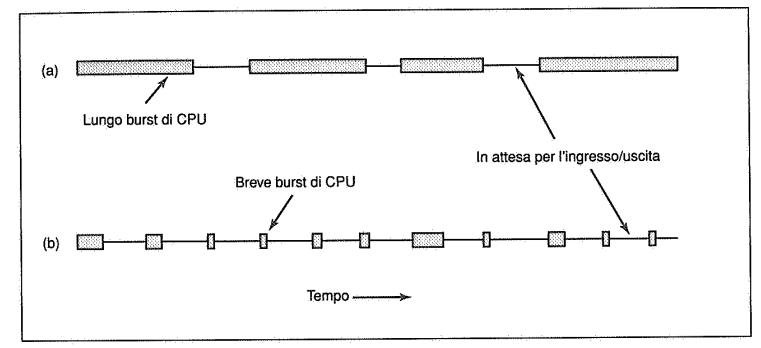
\includegraphics[width=0.6\linewidth]{assets/bound4.png}
    \caption{esempi di processi (a) CPU bound e (b) I/O bound}
\end{figure}

\subsection{Quando schedulare}

Esistono diverse situazioni in cui è utile schedulare, per esempio:
\begin{enumerate}
    \item Creazione di un nuovo processo, si esegue genitore o figlio? Sono entrambi pronti.
    \item Terminazione di un processo, si deve scegliere dalla lista di processi pronti (se non c'è nessuno si esegue il \textit{processo inattivo} fornito dal sistema).
    \item Blocco del processo corrente, per esempio per una richiesta I/O oppure a causa di un \textit{semaforo}.
    \item Interrupt I/O.
\end{enumerate}

Più in generale si deve prendere una decisione ad ogni interruzione di clock, oppure dopo \textit{n} interruzioni.
In base a come gli \textbf{algoritmi di schedulazione} rispondono all'interrupt di clock vengono nominati:
\begin{itemize}
    \item \textbf{nonpreemptive} (senza prerilascio), lascia in esecuzione il processo corrente fino a che non si blocca, non esegue controlli ad ogni clock.
    \item \textbf{preemptive} (con prerilascio), lascia in esecuzione il processo per una quantità prefissata di tempo. 
\end{itemize}

Nel secondo caso lo scheduler prende il controllo alla fine di ogni intervallo di tempo. Se non ci sono clock l'unica possibile soluzione è la prima.

\subsection{Tipi di algoritmi}
Lo scheduler deve ottimizzare cose diverse in base al sistema in questione. In generale riusciamo a dividere i possibili ambienti in tre:
\begin{enumerate}
    \item \textbf{Batch}: non ci sono utenti impazienti.
    \item \textbf{Interattivi}: qui ci sono utenti impazienti, il prerilascio è essenziale.
    \item \textbf{Real time}: a volte il prerilascio non è necessario, spesso i processi in questo ambiente sono costruiti con l'intento di durare il meno possibile. A differenza degli ambienti interattivi qui si eseguono solo programmi che agevolano le applicazioni.
\end{enumerate}

\subsection{Obiettivi}
La maggior parte degli obiettivi dipende dall'ambiente, ma ce ne sono alcuni che sono spesso opportuni.

\begin{figure}[H]
    \centering
    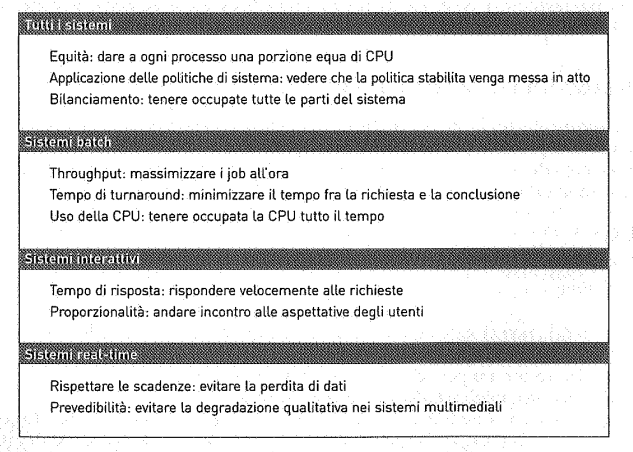
\includegraphics[width=0.6\linewidth]{assets/obiettivi4.png}
    \caption{obiettivi dei diversi sistemi}
\end{figure}


Un generico obiettivo è quello di tenere la CPU il più occupata possibile, idem per i dispositivi di ingresso/uscita. 
I gestori di grossi centri di calcolo che eseguono molti job batch di solito considerano tre metriche per vedere quanto lavorano bene i loro sistemi:
\begin{enumerate}
    \item \textbf{throughput}: il numero di job per ora che il sistema completa.
    \item \textbf{turnaround}: tempo medio dal momento che viene richiesto un job batch fino a che non viene completato.
    \item \textbf{uso della CPU}: parametro abbastanza inutile, è come valutare le auto basandosi sui giri all'ora del motore.
\end{enumerate}

Per i sistemi interattivi, in particolar modo \textit{timesharing} e \textit{server}, è importante minimizzare il \textbf{tempo di risposta}, ovvero il tempo che intercorre tra invio di un comando e arrivo del risultato.

\section{Schedulazione nei sistemi batch}

Alcuni algoritmi sono adeguati sia a sistemi batch che interattivi, di seguito ci concentriamo su quelli adatti ai sistemi batch.

\subsection{First-come First-served}
Senza prerilascio. 

Il primo che arriva viene servito, di seguito gli altri. C'è una coda di processi nello stato di pronto.
Facile da capire e da programmare, equo.

\subsection{Shortest Job First}
Senza prerilascio.

Occorre conoscere in anticipo i tempi di esecuzione.
Quando nella coda si trovano una serie di job di uguale importanza lo scheduler, usando lo \textit{SJF} esegue il più breve.

\begin{figure}[H]
    \centering
    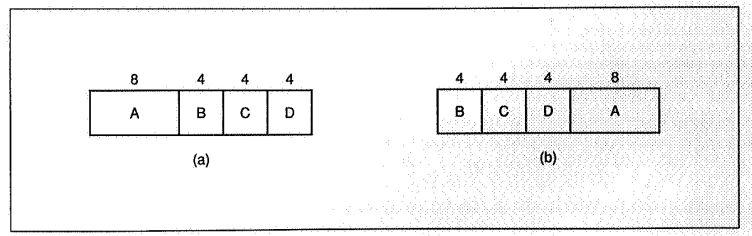
\includegraphics[width=0.6\linewidth]{assets/sjf4.png}
    \caption{coda di processi dello \textit{SJF}}
\end{figure}

Una grossa pecca di questo algoritmo è la necessità di avere tutti i job disponibili contemporaneamente, se un processo breve arriva un istante dopo l'esecuzione di uno lungo si perdono i vantaggi di questo algoritmo.

Un'alternativa al conoscere in anticipo i tempi di esecuzione prevede di stimarli. Per stimare il valore successivo di una serie si utilizza la tecnica dell' \textbf{aging}(invecchiamento), essa si basa sul calcolo della media pesata del valore corrente misurato e la stima precedente: 
\begin{equation}
    T_{st} = \alpha T_{mis} + (1 - \alpha )T_{st}
\end{equation}

\begin{figure}[H]
    \centering
    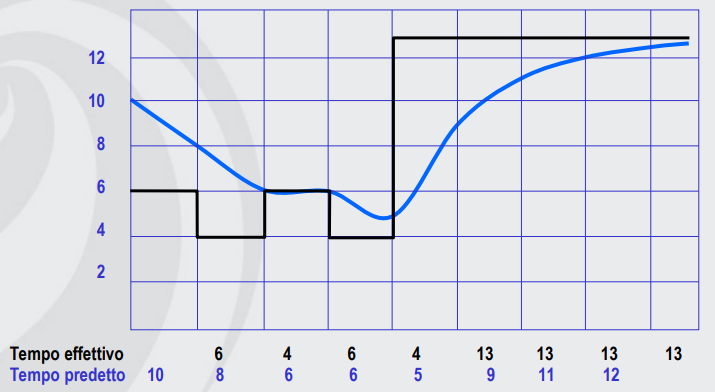
\includegraphics[width=0.6\linewidth]{assets/predizione4.png}
\end{figure}

\subsubsection{Shortest Remaining Time}
Una variante dello \textit{SJF}. Viene eseguito il processo con il tempo \textbf{rimasto} più breve. Anche qui il tempo di esecuzione deve essere noto in anticipo.



\section{Schedulazione nei sistemi interattivi}
Vediamo alcuni algoritmi che possono essere usati nei sistemi interattivi, ma che sono utilizzabili anche nei sistemi batch. 

\subsection{Round Robin}
E' uno degli algoritmi più vecchi, imparziali e semplici.
Ad ogni processo viene assegnato un \textbf{quanto}, durante il quale può essere in esecuzione. Se alla fine del quanto ha ancora bisogno di essere eseguito la CPU viene comunque rilasciata ad un altro processo, allo stesso modo di come si farebbe se finisse la sua esecuzione (o andasse nella lista dei processi \textit{blocked}) prima della fine del quanto.
Lo schedulatore ha bisogno solo di una lista di processi eseguibili.

\begin{figure}[H]
    \centering
    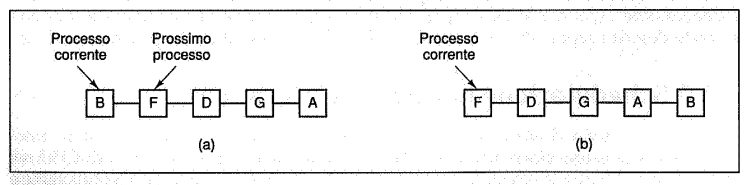
\includegraphics[width=0.6\linewidth]{assets/robin4.png}
    \caption{ }
\end{figure}

La questione interessante è la durata del quanto.
Supponiamo che il \textit{cambio di contesto} impieghi 1 millisecondo, se il quanto è di 4 millisecondi il 20\% del tempo della CPU risulterà sprecato in overhead di gestione ($\frac{1}{1+4}$ = 20\%). Aumentando il quanto la percentuale potrebbe drasticamente diminuire.

Nota che eliminare la prelazione migliorerebbe di parecchio le prestazioni, infatti in quel caso gli scambi di processi sarebbero eseguiti solo quando necessari, ovvero quando un processo si blocca.

Assegnare un quanto troppo breve provoca troppi cambi di contesto, peggiorando l'efficienza della CPU. Assegnare invece quanti troppo lunghi potrebbe provocare tempi di risposta esagerati per richieste interattive brevi.

\subsection{Con priorità}

Ad ogni processo viene assegnata una priorità, viene eseguito il processo che ha la più alta. Per evitare che alcuni processi ad alta priorità rimangano in esecuzione per un tempo indefinito la priorità viene diminuita ad ogni interrupt di clock,.
In alternativa è possibile assegnare un quanto di tempo prefissato come limite massimo, oltre il quale il processo viene bloccato e ne viene mandato un altro in esecuzione, in base alle priorità.

Le priorità possono essere assegnate staticamente o dinamicamente.

\begin{verbatim}
Nota: 
In UNIX "nice" permette ad un utente di diminuire volontariamente la priorità del suo processo.
\end{verbatim}

Un semplice algoritmo, che rende un buon servizio ai processi \textit{I/O bound}, prevede di assegnare priorità uguale ad 1/\textit{f}, dove \textit{f} è la frazione di quanto che un processo ha usato.

Spesso si utilizzano in combinazione i metodi: si assegna una priorità alle classi di processi, e si usa la schedulazione round robin o altre all'interno di ciascuna classe.

\begin{figure}[H]
    \centering
    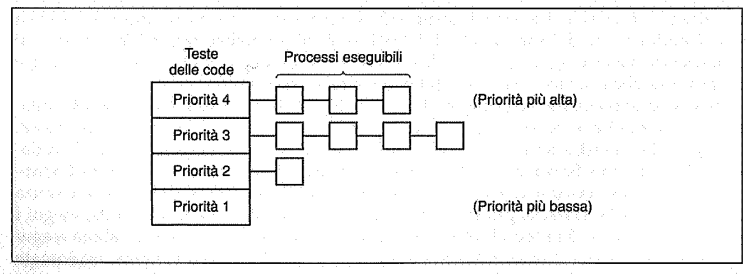
\includegraphics[width=0.6\linewidth]{assets/priorita4.png}
    \caption{ }
    \label{priorita4}
\end{figure}


Un esempio è mostrato in figura \ref{priorita4}. Va notato che se le priorità non vengono aggiornate di sovente, le classi di priorità più bassa possono aspettare troppo tempo.

\subsection{A code multiple}

Questo algoritmo prevede ancora una volta una suddivisione in classi di priorità: i processi appartenenti alla prima vengono eseguiti per un quanto, quelli della seconda per due, quelli della terza per quattro e così via \dots

Ogni volta che un processo viene eseguito per l'intero suo quanto viene spostato ad una classe superiore.
Man mano che un processo sale esso verrà eseguito sempre con minor frequenza, risparmiando tempo di CPU per i processi interattivi brevi.

Ogni coda può usare un algoritmo di scheduling personale. Va fatto uno scheduling anche tra le code.

Per prevenire che un processo inizialmente poco interattivo (e in seguito molto di più) venga punito per sempre sono adottate delle scappatoie, come il reset della priorità dei processi in cui viene premuto il tasto \textit{invio}.

\subsection{Schedulazione garantita}

In questo caso l'approccio è completamente diverso dagli altri, si fa all'utente una promessa, e la si mantiene. Per esempio, se ci sono \textit{n} utenti connessi si promette all'utente che riceverà 1/\textit{n} della potenza della CPU. Stessa cosa vale per i processi.

Per poter adottare questo metodo lo scheduler ha bisogno di tenere traccia di quanta CPU utilizza ciascun processo e rapportare l'informazione con la promessa fatta. Viene definito il \textit{rapporto} di un processo, semplicemente come il rapporto tra tempo di utilizzo della CPU effettivo fratto il tempo di CPU previsto, viene quindi eseguito il processo con il rapporto più basso.

\subsection{Schedulazione a lotteria}

L'idea di base è fornire ai processi dei biglietti della lotteria per varie risorse del sistema, come il tempo di CPU. Ogni volta che deve essere presa una decisione di schedulazione viene scelto a caso un biglietto della lotteria, premiando il processo che lo possiede.

La parte furba della soluzione consiste nel dare più biglietti ai processi più importanti. A lungo andare un processo che detiene una percentuale \textit{p} di biglietti userà una percentuale \textit{p} della risorsa.

Un altro punto importante è che processi cooperativi si possono scambiare i biglietti a piacimento.

\section{Schedulazione nei sistemi real time}

I sistemi real time si dividono in:
\begin{itemize}
    \item \textbf{hard real time systems}
    \item \textbf{soft real time systems}
\end{itemize}

Nei primi è imperativo rispettare le scadenze, nei secondi anche ma è consentita una certa flessibilità all'errore.

In ogni caso il comportamento viene ottenuto dividendo il programma in processi, il cui comportamento è prevedibile e noto in anticipo. Questi processi hanno spesso vita breve e vengono eseguiti nella loro interezza in brevissimo tempo..

Gli eventi di un sistema real time possono essere \textbf{periodici} o \textbf{aperiodici}. 

Nel caso in cui il sistema debba interagire con molti eventi periodici è necessario controllare che la gestione sia fattibile:
ad esempio, se ci sono \textit{m} eventi periodici, l'evento \textit{i}-esimo arriva con periodo P\textsubscript{\textit{i}} e richiede C\textsubscript{\textit{i}} secondi di tempo di CPU per essere gestito, il carico può essere gestito solo se $\sum_{i=1}^{m}{\frac{C_i}{P_i}} \leq 1$.

Un sistema real time che rispetta questo vincolo è detto \textbf{schedulabile}.

In ultimo va sottolineato che i sistemi real time possono essere statici o dinamici, in base a quando prendono le decisioni: nel primo caso le decisioni vengono prese prima che il sistema inizi l'esecuzione. Nel secondo ad esecuzione iniziata. Ovviamente nel primo caso sono necessarie conoscenze a priori.


\section{I livelli di scheduling}

Fino ad ora abbiamo dato per scontato che la memoria principale fosse sufficiente per mantenere tutti i processi da schedulare. Ma che succede se così non fosse?

In questo caso lo scheduling dei processi comporta tempi di switch molto diversi fra processi in memoria principale e di massa.

Un modo pratico di gestire la situazione prevede di utilizzare uno scheduler \textbf{a livelli}.
Esso è diviso in:
\begin{itemize}
    \item scheduler a breve termine: identico a quello visto fino ad ora.
    \item scheduler a medio termine: si occupa degli spostamenti dei processi tra memoria e disco, rimuovendo quelli che sono stati in memoria principale abbastanza e caricando quelli necessari dal disco.
    \item scheduler a lungo termine: sceglie quali job mandare in esecuzione.
\end{itemize}


\begin{figure}[H]
    \centering
    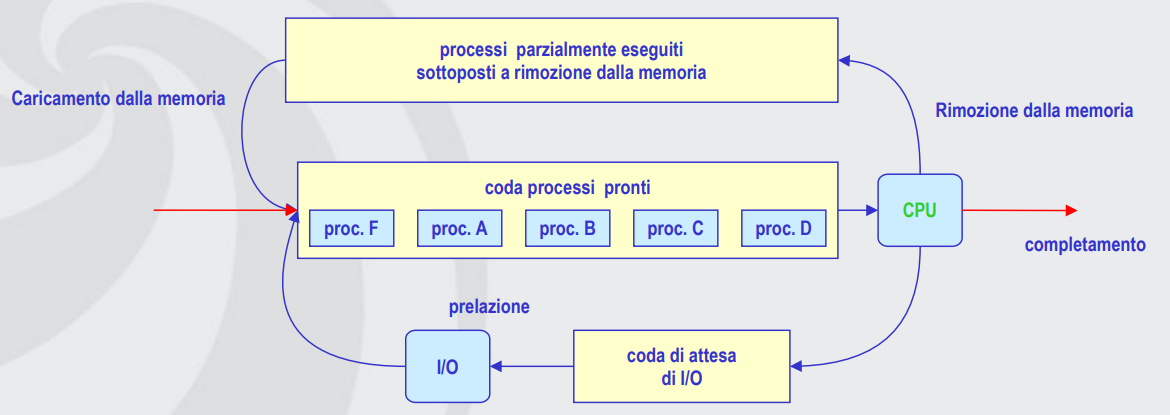
\includegraphics[width=0.9\linewidth]{assets/medio4.png}
    \caption{scheduling a medio termine}
\end{figure}

I criteri utilizzati dallo scheduler di medio termine sono:
\begin{itemize}
    \item il tempo passato dall'ultimo spostamento in memoria.
    \item tempo di CPU assegnato al processo in questione.
    \item grandezza del processo.
    \item priorità del processo.
\end{itemize}

L'algoritmo utilizzato può essere uno di quelli già presentati.

\section{Linux e gli altri..}

Nel kernel Linux 2.6 esistono 140 livelli di priorità, quelli da 0 a 99 sono assegnati ai processi cosiddetti \textit{real time} (non sono realmente real time), e quelli da 100 a 139 per i processi normali.

La \textbf{static priority} si calcola come SP = 120 + \textit{nice}.
Il quanto di tempo invece vale $(140-SP)*20$ \textit{ms} se SP è minore di 120, altrimenti $(140-SP)*5$ \textit{ms}.

Per salvare le informazioni relative ai processi si utilizzano strutture apposite (\textbf{runqueue} e \textbf{prioarray}).


Lo scheduling in Linux kernel 2.4 è diverso da quello presentato, esso sfrutta un concetto simile alla schedulazione a lotteria, usando dei crediti.


In Windows 2000 se ne usa un altro ancora, inoltre in esso i livelli sono 32 e la priorità più alta la hanno i processi dei livelli più alti.

\section{Esercizi}

\dots